\documentclass[10pt,twoside]{article}

\newcommand{\reporttitle}{Mars Rover}
\newcommand{\reportauthor}{}
\newcommand{\reporttype}{Project Report}


% include files that load packages and define macros
%%%%%%%%%%%%%%%%%%%%%%%%%%%%%%%%%%%%%%%%%
% University Assignment Title Page 
% LaTeX Template
% Version 1.0 (27/12/12)
%
% This template has been downloaded from:
% http://www.LaTeXTemplates.com
%
% Original author:
% WikiBooks (http://en.wikibooks.org/wiki/LaTeX/Title_Creation)
%
% License:
% CC BY-NC-SA 3.0 (http://creativecommons.org/licenses/by-nc-sa/3.0/)
% 
% Instructions for using this template:
% This title page is capable of being compiled as is. This is not useful for 
% including it in another document. To do this, you have two options: 
%
% 1) Copy/paste everything between \begin{document} and \end{document} 
% starting at \begin{titlepage} and paste this into another LaTeX file where you 
% want your title page.
% OR
% 2) Remove everything outside the \begin{titlepage} and \end{titlepage} and 
% move this file to the same directory as the LaTeX file you wish to add it to. 
% Then add \input{./title_page_1.tex} to your LaTeX file where you want your
% title page.
%
%----------------------------------------------------------------------------------------
%	PACKAGES AND OTHER DOCUMENT CONFIGURATIONS
%----------------------------------------------------------------------------------------
\usepackage{ifxetex}
\usepackage{textpos}
\usepackage[numbers]{natbib}
\usepackage{kpfonts}
\usepackage[a4paper,hmargin=1.5cm,vmargin=1.5cm,includeheadfoot]{geometry}
\usepackage{ifxetex}
\usepackage{stackengine}
\usepackage{tabularx,longtable,multirow,subfigure,caption}%hangcaption
\usepackage{fncylab} %formatting of labels
\usepackage{fancyhdr}
\usepackage{color}
\usepackage[tight,ugly]{units}
\usepackage{url}
\usepackage{float}
\usepackage[english]{babel}
\usepackage{amsmath}
\usepackage{graphicx}
\usepackage[colorinlistoftodos]{todonotes}
\usepackage{dsfont}
\usepackage{epstopdf} % automatically replace .eps with .pdf in graphics
\usepackage{backref}
\usepackage{array}
\usepackage{latexsym}
\usepackage{etoolbox}
\usepackage{tikz}
\usepackage{multirow}
\usepackage{booktabs}
\usepackage[toc,page]{appendix}
\usepackage{listings}
\usepackage{xfrac}
\usepackage{titlesec}
%\usepackage{enumerate} % for numbering with [a)] format 
\setlength{\parskip}{1em}

%%%%%%%%%% SAM VERILOG %%%%%%%%%%%%%%%%%%%%%%

\usepackage{minted}
\usemintedstyle{manni}  %manni

%%%%%%%%%%%%%%%%%%%%%%%%%%%%%%%%%%%%%%%%%%%%%%

\ifxetex
\usepackage{fontspec}
\setmainfont[Scale=.8]{OpenDyslexic-Regular}
\else
\usepackage[pdftex,pagebackref,hypertexnames=false,colorlinks]{hyperref} % provide links in pdf
\hypersetup{pdftitle={},
  pdfsubject={}, 
  pdfauthor={\reportauthor},
  pdfkeywords={}, 
  pdfstartview=FitH,
  pdfpagemode={UseOutlines},% None, FullScreen, UseOutlines
  bookmarksnumbered=true, bookmarksopen=true, colorlinks,
    citecolor=black,%
    filecolor=black,%
    linkcolor=black,%
    urlcolor=black}
\usepackage[all]{hypcap}
\fi

\usepackage{tcolorbox}

% various theorems
\usepackage{ntheorem}
\theoremstyle{break}
\newtheorem{lemma}{Lemma}
\newtheorem{theorem}{Theorem}
\newtheorem{remark}{Remark}
\newtheorem{definition}{Definition}
\newtheorem{proof}{Proof}

% example-environment
\newenvironment{example}[1][]
{ 
\vspace{4mm}
\noindent\makebox[\linewidth]{\rule{\hsize}{1.5pt}}
\textbf{Example #1}\\
}
{ 
\noindent\newline\makebox[\linewidth]{\rule{\hsize}{1.0pt}}
}



%\renewcommand{\rmdefault}{pplx} % Palatino
% \renewcommand{\rmdefault}{put} % Utopia

\ifxetex
\else
\renewcommand*{\rmdefault}{bch} % Charter
\renewcommand*{\ttdefault}{cmtt} % Computer Modern Typewriter
%\renewcommand*{\rmdefault}{phv} % Helvetica
%\renewcommand*{\rmdefault}{iwona} % Avant Garde
\fi

\setlength{\parindent}{0em}  % indentation of paragraph

\setlength{\headheight}{14.5pt}
\pagestyle{fancy}
\fancyfoot[ER,OL]{\thepage}%Page no. in the left on
                                %odd pages and on right on even pages
\fancyfoot[OC,EC]{\sffamily }
\renewcommand{\headrulewidth}{0.1pt}
\renewcommand{\footrulewidth}{0.1pt}
\captionsetup{margin=10pt,font=small,labelfont=bf}


%--- chapter heading

\def\@makechapterhead#1{%
  \vspace*{10\p@}%
  {\parindent \z@ \raggedright %\sffamily
        %{\Large \MakeUppercase{\@chapapp} \space \thechapter}
        %\\
        %\hrulefill
        %\par\nobreak
        %\vskip 10\p@
    \interlinepenalty\@M
    \Huge \bfseries 
    \thechapter \space\space #1\par\nobreak
    \vskip 30\p@
  }}

%---chapter heading for \chapter*  
\def\@makeschapterhead#1{%
  \vspace*{10\p@}%
  {\parindent \z@ \raggedright
    \sffamily
    \interlinepenalty\@M
    \Huge \bfseries  
    #1\par\nobreak
    \vskip 30\p@
  }}
  



% %%%%%%%%%%%%% boxit
\def\Beginboxit
   {\par
    \vbox\bgroup
	   \hrule
	   \hbox\bgroup
		  \vrule \kern1.2pt %
		  \vbox\bgroup\kern1.2pt
   }

\def\Endboxit{%
			      \kern1.2pt
		       \egroup
		  \kern1.2pt\vrule
		\egroup
	   \hrule
	 \egroup
   }	

\newenvironment{boxit}{\Beginboxit}{\Endboxit}
\newenvironment{boxit*}{\Beginboxit\hbox to\hsize{}}{\Endboxit}



\allowdisplaybreaks

\makeatletter
\newcounter{elimination@steps}
\newcolumntype{R}[1]{>{\raggedleft\arraybackslash$}p{#1}<{$}}
\def\elimination@num@rights{}
\def\elimination@num@variables{}
\def\elimination@col@width{}
\newenvironment{elimination}[4][0]
{
    \setcounter{elimination@steps}{0}
    \def\elimination@num@rights{#1}
    \def\elimination@num@variables{#2}
    \def\elimination@col@width{#3}
    \renewcommand{\arraystretch}{#4}
    \start@align\@ne\st@rredtrue\m@ne
}
{
    \endalign
    \ignorespacesafterend
}
\newcommand{\eliminationstep}[2]
{
    \ifnum\value{elimination@steps}>0\leadsto\quad\fi
    \left[
        \ifnum\elimination@num@rights>0
            \begin{array}
            {@{}*{\elimination@num@variables}{R{\elimination@col@width}}
            |@{}*{\elimination@num@rights}{R{\elimination@col@width}}}
        \else
            \begin{array}
            {@{}*{\elimination@num@variables}{R{\elimination@col@width}}}
        \fi
            #1
        \end{array}
    \right]
    & 
    \begin{array}{l}
        #2
    \end{array}
    &%                                    moved second & here
    \addtocounter{elimination@steps}{1}
}
\makeatother

%% Fast macro for column vectors
\makeatletter  
\def\colvec#1{\expandafter\colvec@i#1,,,,,,,,,\@nil}
\def\colvec@i#1,#2,#3,#4,#5,#6,#7,#8,#9\@nil{% 
  \ifx$#2$ \begin{bmatrix}#1\end{bmatrix} \else
    \ifx$#3$ \begin{bmatrix}#1\\#2\end{bmatrix} \else
      \ifx$#4$ \begin{bmatrix}#1\\#2\\#3\end{bmatrix}\else
        \ifx$#5$ \begin{bmatrix}#1\\#2\\#3\\#4\end{bmatrix}\else
          \ifx$#6$ \begin{bmatrix}#1\\#2\\#3\\#4\\#5\end{bmatrix}\else
            \ifx$#7$ \begin{bmatrix}#1\\#2\\#3\\#4\\#5\\#6\end{bmatrix}\else
              \ifx$#8$ \begin{bmatrix}#1\\#2\\#3\\#4\\#5\\#6\\#7\end{bmatrix}\else
                 \PackageError{Column Vector}{The vector you tried to write is too big, use bmatrix instead}{Try using the bmatrix environment}
              \fi
            \fi
          \fi
        \fi
      \fi
    \fi
  \fi 
}  
\makeatother

\robustify{\colvec}

%%% Local Variables: 
%%% mode: latex
%%% TeX-master: "notes"
%%% End: 
 % various packages needed for maths etc.
% quick way of adding a figure
\newcommand{\fig}[3]{
 \begin{center}
 \scalebox{#3}{\includegraphics[#2]{#1}}
 \end{center}
}

%\newcommand*{\point}[1]{\vec{\mkern0mu#1}}
\newcommand{\ci}[0]{\perp\!\!\!\!\!\perp} % conditional independence
\newcommand{\point}[1]{{#1}} % points 
\renewcommand{\vec}[1]{{\boldsymbol{{#1}}}} % vector
\newcommand{\mat}[1]{{\boldsymbol{{#1}}}} % matrix
\newcommand{\R}[0]{\mathds{R}} % real numbers
\newcommand{\Z}[0]{\mathds{Z}} % integers
\newcommand{\N}[0]{\mathds{N}} % natural numbers
\newcommand{\nat}[0]{\mathds{N}} % natural numbers
\newcommand{\Q}[0]{\mathds{Q}} % rational numbers
\ifxetex
\newcommand{\C}[0]{\mathds{C}} % complex numbers
\else
\newcommand{\C}[0]{\mathds{C}} % complex numbers
\fi
\newcommand{\tr}[0]{\text{tr}} % trace
\renewcommand{\d}[0]{\mathrm{d}} % total derivative
\newcommand{\inv}{^{-1}} % inverse
\newcommand{\id}{\mathrm{id}} % identity mapping
\renewcommand{\dim}{\mathrm{dim}} % dimension
\newcommand{\rank}[0]{\mathrm{rk}} % rank
\newcommand{\determ}[1]{\mathrm{det}(#1)} % determinant
\newcommand{\scp}[2]{\langle #1 , #2 \rangle}
\newcommand{\kernel}[0]{\mathrm{ker}} % kernel/nullspace
\newcommand{\img}[0]{\mathrm{Im}} % image
\newcommand{\idx}[1]{{(#1)}}
\DeclareMathOperator*{\diag}{diag}
\newcommand{\E}{\mathds{E}} % expectation
\newcommand{\var}{\mathds{V}} % variance
\newcommand{\gauss}[2]{\mathcal{N}\big(#1,\,#2\big)} % gaussian distribution N(.,.)
\newcommand{\gaussx}[3]{\mathcal{N}\big(#1\,|\,#2,\,#3\big)} % gaussian distribution N(.|.,.)
\newcommand{\gaussBig}[2]{\mathcal{N}\left(#1,\,#2\right)} % see above, but with brackets that adjust to the height of the arguments
\newcommand{\gaussxBig}[3]{\mathcal{N}\left(#1\,|\,#2,\,#3\right)} % see above, but with brackets that adjust to the height of the arguments
\DeclareMathOperator{\cov}{Cov} % covariance (matrix) 
\ifxetex
\renewcommand{\T}[0]{^\top} % transpose
\else
\newcommand{\T}[0]{^\top}
\fi
% matrix determinant
\newcommand{\matdet}[1]{
\left|
\begin{matrix}
#1
\end{matrix}
\right|
}



%%% various color definitions
\definecolor{darkgreen}{rgb}{0,0.6,0}

\newcommand{\blue}[1]{{\color{blue}#1}}
\newcommand{\red}[1]{{\color{red}#1}}
\newcommand{\green}[1]{{\color{darkgreen}#1}}
\newcommand{\orange}[1]{{\color{orange}#1}}
\newcommand{\magenta}[1]{{\color{magenta}#1}}
\newcommand{\cyan}[1]{{\color{cyan}#1}}


% redefine emph
\renewcommand{\emph}[1]{\blue{\bf{#1}}}

% place a colored box around a character
\gdef\colchar#1#2{%
  \tikz[baseline]{%
  \node[anchor=base,inner sep=2pt,outer sep=0pt,fill = #2!20] {#1};
    }%
}%
 % short-hand notation and macros
\setcounter{tocdepth}{2}    % Makes contents smaller
\graphicspath{ {figures/} }

\begin{document}

% Last modification: 2016-09-29 (Marc Deisenroth)
\begin{titlepage}

\newcommand{\HRule}{\rule{\linewidth}{0.5mm}} % Defines a new command for the horizontal lines, change thickness here


%----------------------------------------------------------------------------------------
%	LOGO SECTION
%----------------------------------------------------------------------------------------


    \begin{tikzpicture}[remember picture,overlay]
    \node[anchor=north west,inner sep=1cm] at (current page.north west)
          {
\includegraphics[width = 4cm]{./figures/imperial}\\[0.5cm] };
    \end{tikzpicture}


\begin{center} % Center remainder of the page

%----------------------------------------------------------------------------------------
%	HEADING SECTIONS
%----------------------------------------------------------------------------------------
\textsc{\LARGE \reporttype}\\[1.5cm] 
\textsc{\Large Imperial College London}\\[0.5cm] 
\textsc{\large Department of Electrical and Electronic Engineering}\\[0.5cm] 
%----------------------------------------------------------------------------------------
%	TITLE SECTION
%----------------------------------------------------------------------------------------

\HRule \\[0.4cm]
{ \huge \bfseries \reporttitle}\\ % Title of your document
\HRule \\[1.5cm]
\end{center}
%----------------------------------------------------------------------------------------
%	AUTHOR SECTION
%----------------------------------------------------------------------------------------

%\begin{minipage}{0.4\hsize}
\begin{center}
\textbf{Authors:}\\
Sam Taylor - 01705109\\
Martin Prusa - 01713176\\
Leonardo Garofalo - 01746454\\
Katherine Zhang - 01504365\\
Maximus Wickham - 01717673\\
Matilde Piccoli - 01764158 \\
\end{center}
\vspace{2cm}
\makeatletter
\centering
Date: \@date 

\vfill % Fill the rest of the page with whitespace



\makeatother


\end{titlepage}



\newpage

\tableofcontents

\newpage
\section{Abstract}

\newpage
\section{Project Management}

The given timeline for the project was 5 weeks. The first week was allocated for research and planning. Each member carried out research on their own module and a meeting was held to identify the main tasks and create a tentative project timeline. From the second week on-wards, bi-weekly meetings were held: one meeting at the beginning of the week to set the targets for that week and one meeting in the middle of the week to check up on progress. Week 2 was planned to work on the basic functionalities for each module so that a very basic prototype of the rover could be put together. In week 3, more sophisticated implementations and additional functions were added. By the end of week 4, the design of each module was finalised and integration of the whole rover was completed. The final week of the project was used to clean up any issues with the integrated rover and make final adjustments. 

\textbf{Meeting Structure:}

At the beginning of each week we held a 45 minute meeting. Each member would take 5 minutes to update the group on their progress on the targets set for the previous week, discuss any issues they found and set new targets for the week. Midway through the week we had a brief 20 minute meeting to check in on everyone’s progress and give the opportunity for the members to bring up any problems or difficulties they might have ran into and adjust plans accordingly.

\textbf{Tools Used for Project Management:}

A Gantt chart was used to illustrate the main tasks to be completed for each module and set deadlines for their completion. It served as an effective method for tracking progress and keeping on track.

\begin{figure}[hbt]
    \centering
    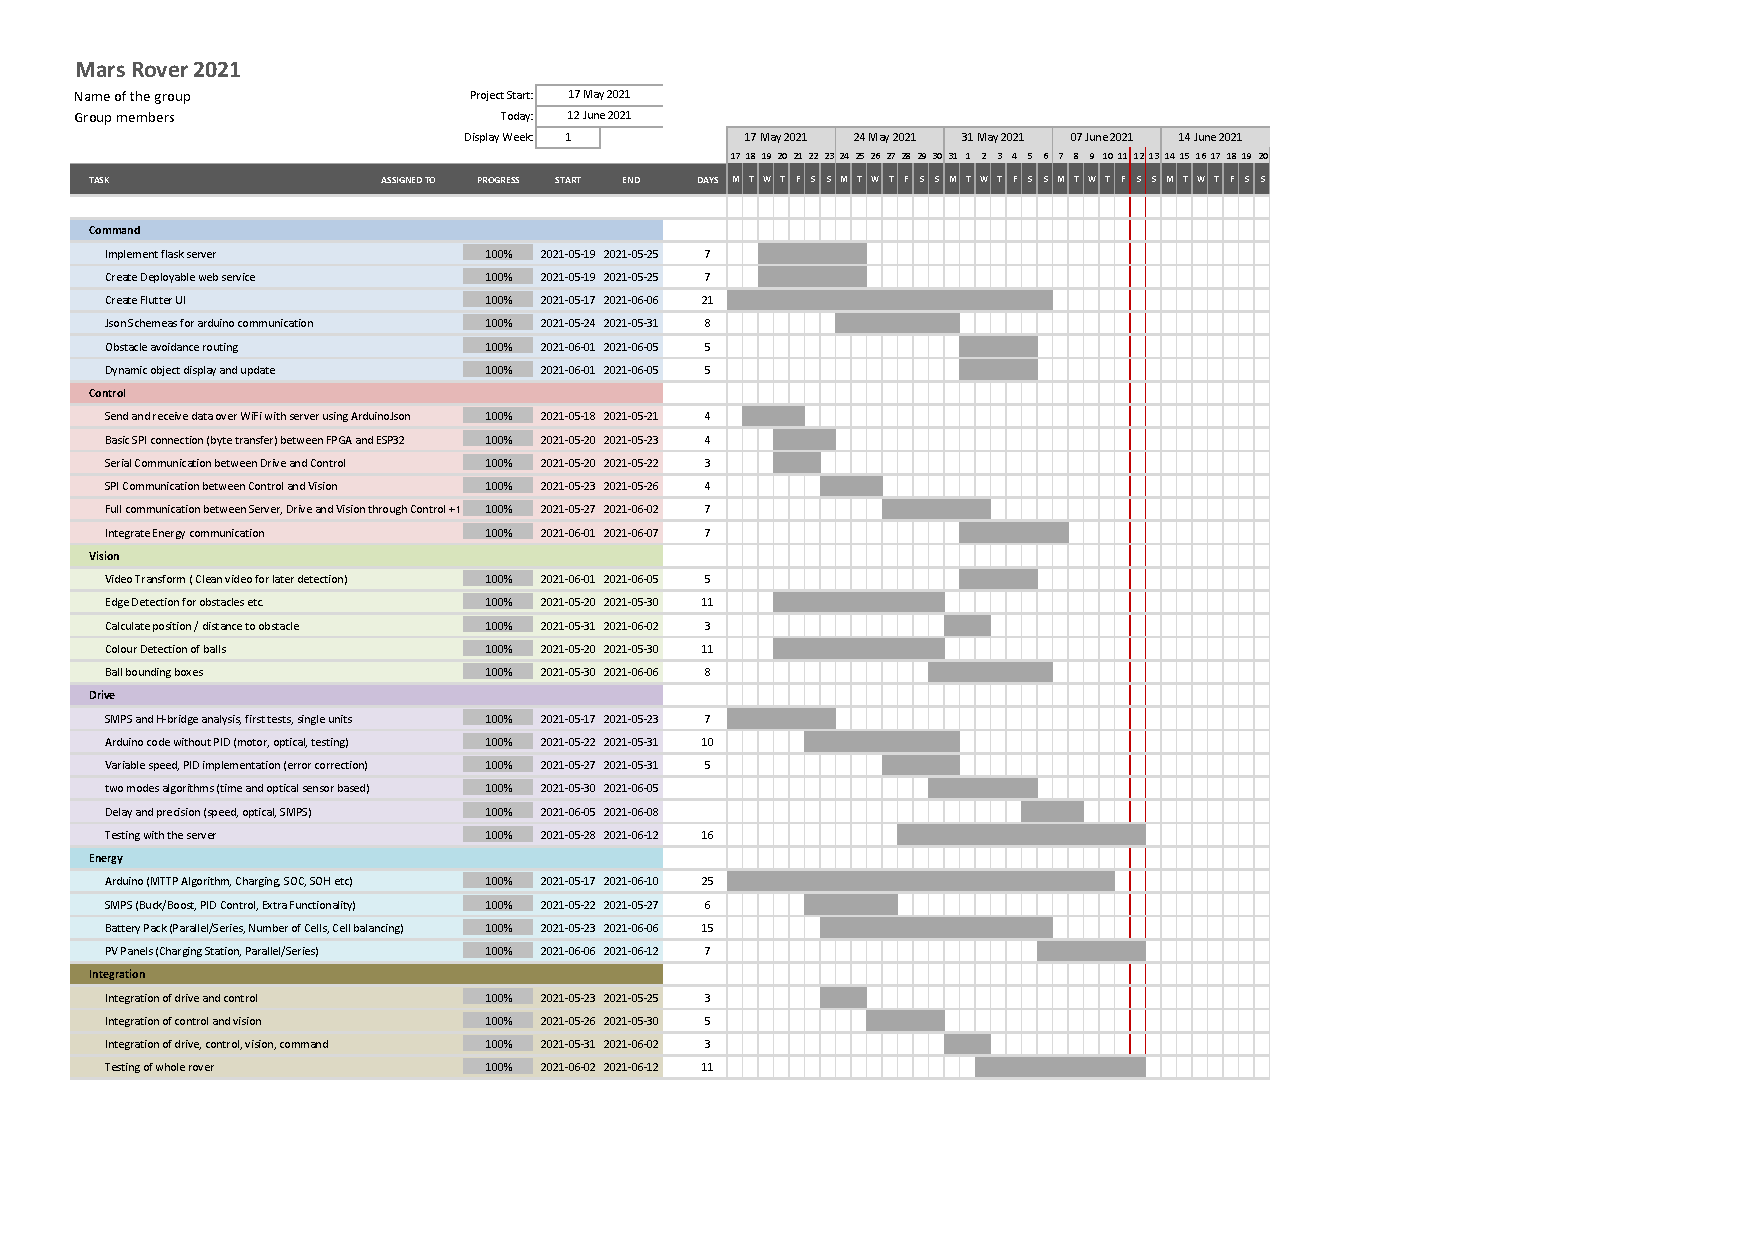
\includegraphics[scale = 0.66,trim={1cm 3cm 8cm 0},clip]{GanttChart.pdf}
    \caption{Gantt Chart}
    \label{fig:GanttChart}
\end{figure}

The productivity software Notion was also used for each member to make notes of their initial design process, development and testing. It provided an easy method to share progress with the rest of the team. The shared calendar was used to set dates of meetings and mark internal deadlines. Git was used for version control.

\newpage
\section{Design Process}
\subsection{Structural and Functional Design}
\subsection{Problem Definition and Design Criteria}

\subsubsection{Drive}

\subsubsection{Energy}
The energy subsystem can be split into 4 top level sections which all combine to provide battery power and charging to the rover. These can then be broken down into smaller subsections which are more manageable and easier to test individually (Table \ref{tab:EnergySpec}). This also allows for more unique features to be added later on in the process. 

\begin{table}[htp]
\renewcommand{\arraystretch}{1.3}
 \centering
\begin{tabular}{@{}cll@{}}
\toprule
\multicolumn{1}{l}{Section}                       & Criteria          & Description \\ \midrule
\multirow{8}{*}{Arduino}                          & Data Collection   & \parbox{0.61\linewidth}{The current and voltage should be recorded continuously for safety features}            \\
                                                  & Charge Strategy   & \parbox{0.61\linewidth}{Try to get near maximum possible capacity out of cells}            \\
                                                  & SOC Estimation    &  \parbox{0.61\linewidth}{Real time percentage capacity of the battery via coulomb counting}           \\
                                                  & SOH Maintenance   &  \parbox{0.61\linewidth}{Provide balancing of the cells and an estimation of the SOH}           \\
                                                  & PV MPPT algorithm &  \parbox{0.61\linewidth}{Get the maximum amount of power out of the PV Panels}           \\
                                                  & Communication     & \parbox{0.61\linewidth}{Transmit and receive data from Control}            \\
                                                  & Cell Safety    & \parbox{0.61\linewidth}{$I_{In}^{Max} = 250mA$, $I_{Out}^{Max} = 500mA$, $V_{Bat}^{Max} = 3.7V$, $V_{Bat}^{Min} = 2.3V$}            \\
                                                  & Rover Range     & 
                                                  \parbox{0.61\linewidth}{Work out Rover range from Drive current and speed} \\\midrule
\multicolumn{1}{l}{{\multirow{3}{*}{SMPS}}}       & Charging Buck/Boost        & \parbox{0.61\linewidth}{PV voltage                                                         stepped down to battery voltage}            \\
                                                  & Discharging Buck/Boost    & \parbox{0.61\linewidth}{Battery voltage stepped down to motor control voltage} \\ 
                                                  & Drive Current Required &
                                                  \parbox{0.61\linewidth}{$I_{Drive}^{Max}$ = 550mA} \\ \midrule
\multicolumn{1}{l}{\multirow{2}{*}{Battery Pack}} & Number of Cells   &  \parbox{0.61\linewidth}{2}           \\
\multicolumn{1}{l}{}                              & Configuration     & \parbox{0.61\linewidth}{Series to allow to better current limitation}            \\ \midrule
\multicolumn{1}{l}{{\multirow{3}{*}{PV Panels}}}                     & Configuration     &  \parbox{0.61\linewidth}{2x2 (Two in series then in parallel)}           \\ 
                                                  & Usage &
                                                  \parbox{0.61\linewidth}{A charging station setup in a sunlit area} \\ \bottomrule
\end{tabular}
\caption{\label{tab:EnergySpec} Energy Specification}
\end{table}

\textbf{Design Philosophy}

The energy subsection would require a lot of initial research into lithium based cells (LiFePO cells were provided) as these have never been covered as a module. A document was made which collated the various amounts of research into cell charging/discharging, safety and PV panels. Then a process of simple testing ensued to characterise some of the cells and PV panels. After this was finished, the direction to take became clearer and work based upon Gantt diagram (\ref{fig:GanttChart}) began. The aim was to investigate the variety of options available which would allow me to pick and choose the best. This did lead to a number of dead-ends but in many cases a lot was learned from these and subsequently improved on the overall design.

Due to the large amounts of code required for testing, a number of files were made which would be uploaded to Github. A final Arduino program was made towards the end of the project which could combine all the functions from the various files. These will have been individually tested to ensure they work. Ideally a final test would also be performed but due to possible defects in the cell supply, this was never realised.

\newpage


\subsubsection{Vision}
The function of the vision system was broken into three general objectives of which the team agreed the vision system should achieve (See objectives below) .We agreed aspects like rover position and path finding would be better tackled by different subsystems. The following diagram shows the three main functions of Vision.

\begin{figure}[hbt!]
    \centering
    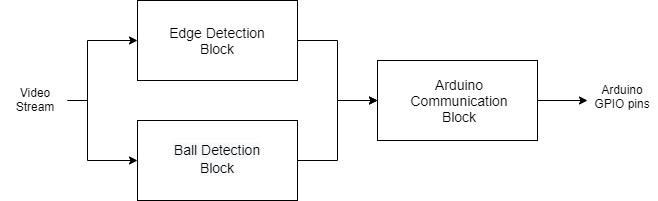
\includegraphics[scale=0.35]{HighLevelDesign.jpg}
    \captionsetup{justification=centering}
    \caption{High Level Block diagram}
\end{figure}

\smallbreak
After this high-level design i broke down each High level objective into a series of smaller objectives with several criteria which the subsystem would have to be meet to successfully accomplish its highlevel functionality. 
\smallbreak
\textbf{Ball detection:}

The diagram outlines a basic strategy for approaching the detection of balls through a process of highlighting , filtering and calculating. Each  ball occupies its own spectrum of colours in varying brightness conditions this spectrum can be highlighted so that we determine the maximum and minimum pixels of balls.Each block was designed to be testable by certain criteria so its success can be verified to ensure the entire block is functioning. 

\textbf{Edge detection:}

Calculating the luminance space of the image we can observe the brightness of each pixel which after the
application of a Sobel filter can be used to produce the edge space. This edge space can then be highlighted
using a threshold this highlighted space will reveal edges. .Each block was designed to be testable by certain
criteria so its success can be verified to ensure the entire block is functioning.

\textbf{Communication:}

This block facilitates communication between the Arduino ESP connected to the FPGA pins.It will utilise an agreed method to transfer data one way to the Control subsystem. All variables calculated in the analysis of the vision data will be relayed to it.


\begin{figure}[!htb]
    \centering
    \begin{minipage}{.33\textwidth}
        \centering
        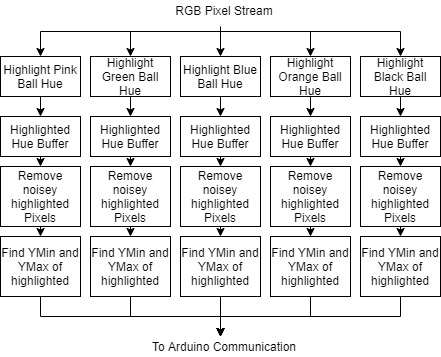
\includegraphics[width=0.8\linewidth, height=0.2\textheight]{BallDetection.jpg}
        \caption{Ball detection overview}
        \label{fig:BallDetectionOverview}
    \end{minipage}%
    \begin{minipage}{0.33\textwidth}
        \centering
        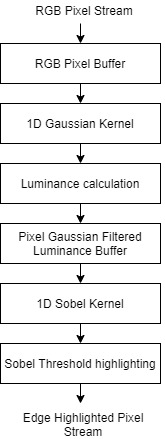
\includegraphics[width=0.4\linewidth, height=0.25\textheight]{EdgeDetection.jpg}
        \caption{Edge detection overview}
        \label{fig:EdgeDetectionOverview}
    \end{minipage}%
    \begin{minipage}{.33\textwidth}
        \centering
        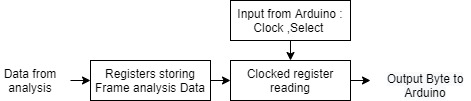
\includegraphics[width=1\linewidth, height=0.08\textheight]{ArduinoComms.jpg}
        \caption{Arduino Comms overview}
        \label{fig:ArduinoComms}
    \end{minipage}%
\end{figure}


\newpage


\textbf{Leaving us with the final design criteria list as such :}

\begin{enumerate}
\itemsep0em
  \item Detect All five balls independently. 
        \begin{enumerate}
            \itemsep-0.2em
            \item Consistently highlight pixels belonging to balls in a plain environment.
                \begin{enumerate}
                    \itemsep-0.2em
                    \item Highlight ball in multiple levels of brightness
                    \item Highlight the intended colour of ball and no others.
                    \item Eliminate (Do not highlight) the environment that is not the intended ball.
                \end{enumerate}
            \item Filter/Ignore noise data that may exist in the image.
                \begin{enumerate}
                    \itemsep-0.2em
                    \item Successfully remove any data that has been highlighted incorrectly when isolating the ball. 
                    \item Successfully avoid removing the correctly highlighted pixels of the ball.
                \end{enumerate}
            \item Accurately find minimum and maximum bounds for balls in the environment .
                \begin{enumerate}
                    \itemsep-0.2em
                    \item Ensure associated Ymin and Ymax are accurate through visual confirmation. 
                    \item Update Ymin and Ymax accordingly with each frame 
                \end{enumerate}
            \item Calculate distance to from ball to rover from image. 
                \begin{enumerate}
                    \itemsep-0.2em
                    \item Calculate the distance from rover to ball within 5\verb|%| of real distance 
                \end{enumerate}
        \end{enumerate}
  \item Detect obstructions of unknown visual data .
        \begin{enumerate}
            \itemsep-0.2em
            \item Applying filtering to reveal edges in image.
                \begin{enumerate}
                    \itemsep-0.2em
                    \item Reveal all Horizontal edges in an image through highlighting confirm visually
                    \item Extract meaningful depth data from highlighted edges. 
                \end{enumerate}
            \item Calculate the distance to edges from past and present image data.
                 \begin{enumerate}
                    \itemsep-0.2em
                    \item Reveal all Horizontal edges in an image through highlighting confirm visually
                    \item Extract meaningful depth data from highlighted edges. 
                    \item Store depth data to be outputted sent to control subsystem for analysis
                \end{enumerate}
        \end{enumerate}
  \item Relay information on detected objects to Control subsystem for further processing.
        \begin{enumerate}
            \itemsep-0.2em
            \item Instantiate a memory that can store all data of from analysis of current frame. 
            \item Relay data gathered and calculated in an agreed format to Control subsystem.
            \item Check relayed data is accurately received on the Command / Control subsystem. 
        \end{enumerate}
\end{enumerate}

\textbf{My development philosophy / process was the following:}

I aimed to recursively improve my design and implementation to ensure a robust and flexible subsystem that could adapt to any new criteria , tests or functionality the team agreed upon as the project progressed. This meant i would follow a development cycle illustrated below.

\begin{figure}[hbt!]
    \centering
    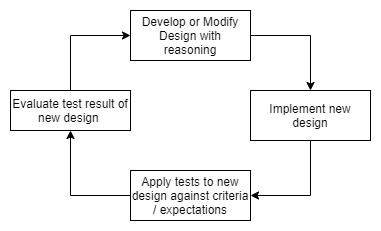
\includegraphics[scale=0.60]{FlowOfDesign.jpg}
    \captionsetup{justification=centering}
    \caption{Subsystem Development Process}
\end{figure}

The development of my system would all take place upon the DE-10 FPGA and camera provided based on the demo project provided. All development was limited to the EEEImgProc.v file where i implemented all verilog code necessary to meet my design requirements. Any hardware utilised was initialised here or modified in the project QSYS. I aimed on utilising minimal hardware/implementations to develop  my subsytem meaning i often implemented designs in verilog rather than choosing pre-existing library hardware. This was done to reduce issues when debugging and ensure i was not incorporating functionality that was not necessary in my subsystem.




\newpage


\subsubsection{Command}
The rover command module was designed to provide two main functions. Firstly, it had to provide an interface to allow the user to send commands to the rover in different formats and provide information back to the user with regard to the rovers position and sensor data. Secondly, the module had to provide drive commands to the rover based on the user input and on the vision data sent to it from the rover. 
\smallbreak
The different types of commands that we decided to allow the user to send are as follows:
\begin{enumerate}
  \item Commands in the form of a coordinate relative to the rovers current position, with the rover deciding the best route to reach the destination.
  \item Direct commands such as move forward and turn that the rover follows exactly.
  \item Commands to move to a given ball and search for it if it's position is unknown. 
\end{enumerate}
The information that would be sent back to the user can be broken down as follows:
\begin{enumerate}
  \item Provide visual indication of the position of any detected balls relative to the rover position.
  \item Provide and indication of the current charge and battery health of the rover.
  \item Provide a list of the commands the rover still has to complete.
  \item Display the current drive mode that the rover is in.
  \item Display depth data for any object in front of the rover.
\end{enumerate}
In order to allow this requirements to be filled it a map based system was decided upon, this would allow the user to easily click on a position that they desired the rover to move to whilst also displaying the current position of any balls within the same format. In order to allow for commands to be entered a textual input format would also be needed. In addition to ball detection we also decided to try and find some way of estimating the depth in front of the rover to any obstacle using the difference between two successive frames. It was unclear at the beginning of the project however if this would be possible.
\smallbreak
When calculating the actual commands to send to the rover the command module would use three different modes.
\begin{enumerate}
  \item Map mode: In this mode the rover would be sent a small movement to take it towards the target coordinate. This movement would incorporate obstacle avoidance for any balls in the rovers path.
  \item Command mode: In this mode the rover would be sent a small movement that would be a division of a command sent by the user. The rover would be continuously sent these incremental commands as it completed them until the entire user command was completed.
  \item Search mode: In this mode the rover would be searching for a given ball, if the balls position was node the same method as map mode would be used, with the ball as the target location. If the balls position was unknown a searching route would have to be implemented instead.
\end{enumerate}
It was decided that whenever the rover completed a movement sent to it from command it would send back its change in position and orientation along with any sensor data, this would allow the command module to calculate the new command to send the rover.


\subsubsection{Control}

The Control subsystem main task is to allow fast and efficient data exchange between the server and the rover. This process can be broken down in:
\begin{itemize}
    \item collect processed data provided by the relevant subsystems
    \item send the collected data to the server for analysis
    \item receive data back from the server and forward it to the relevant subsystems
\end{itemize}

The control subsystem needs to communicate with every other subsystem via a suitable communication protocol. The communication protocol was selected taking into account the amount of data that each subsystem needs to send and the design requirements chosen for the rover. %%%order to satisfy the design requirements chosen for the other subsystems.

\begin{center}
\begin{tabular}{ |c|c|c|c| } 
\hline
Subsystem & Data exchanged & Payload size & Communication mode \\
\hline
\multirow{1}{4em}{Vision} & processed image data & large & unidirectional $\vert$ Vision $\rightarrow$ Control \\ 

\multirow{1}{4em}{Drive} & position data & small & bidirectional $\vert$ Drive $\leftrightarrow$ Control \\ 

\multirow{1}{4em}{Energy} & battery data & small & bidirectional $\vert$ Energy $\leftrightarrow$ Control \\ 

\multirow{1}{4em}{Command} & Energy, Drive and Vision data & very large & bidirectional $\vert$ Command $\leftrightarrow$ Control \\



\hline
\end{tabular}
\end{center}




The Control subsystem task is to provide fast and reliable data
transfer between the different subsystems. 
\medskip

In particular, the Control subsyem aim is to 

This task can broken into smaller sub-tasks:
\begin{itemize}
    \item communication with the Command subsystem
    \item communication with the Drive subsystem
    \item communication with the Vision subsystem
    \item communication with the Energy subsystem
\end{itemize}





It was decided that that the Energy subsystem should not only be able to send information but also to receive it. Sending data to Energy is not shown in the diagram and happens in parallel with the main flow of information. The details are discussed in the Control Implementation section.

\paragraph{Command communication}
The Command subsystem needs to easily extract and manipulate the data sent from the Esp32. For this reason we decided to make use of JSON documents as our file format for data interchange. Communication with the Command subsystem (server) exploits WiFi connection and http requests.
%justify why you picked http
%talk about JSON objects

\paragraph{Vision communication}
The Vision subsystem needs to send large amount of processed image data to the server. For this reason the communication protocol that we picked was SPI as it's the fastest protocol that esp32 supports

\paragraph{Drive and Energy communication}
The Drive and Energy subsystems both send and receive data from the server. Since only a very small amount of data is exchanged between the esp32 and Drive or Energy, and since the esp32 supports distinct 2 UART ports, the communication protocol that we picked was UART

\begin{figure}[hbt!]
    \centering
    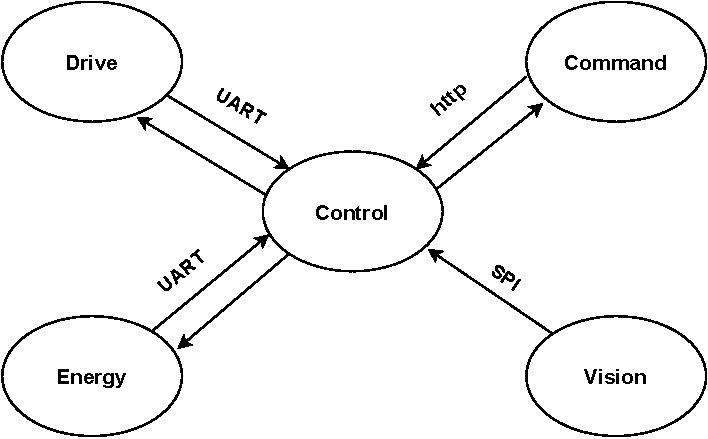
\includegraphics[scale=0.40]{esp32_comms.pdf}
    \captionsetup{justification=centering}
    \caption{communication protocols}
\end{figure}

\newpage
\subsubsection{Integration}

\newpage

\section{Design Implementation}

\subsection{Drive}

\subsection{Energy}
\textbf{Arduino - Data Collection}

Upon initial testing of the Arduino, it became clear that the analogue inputs fluctuate significantly. To mitigate this in both the current and voltage, a 'moving average' filter was implemented which took the 1000 values before the slow loop and summed them in a cumulative variable. This was then divided by 1000 to get the average.

\textbf{Arduino - Charge Strategy}

To get the most capacity out of a single cell, a CC/CV (Constant Current/ Constant Voltage) charge strategy was decided upon. This involves charging a cell with a steady current until the maximum voltage is reached. Both the charging current and maximum voltage are dictated by the data sheet of the cell in use (Appendix \ref{appendix:Energy}.\ref{fig:CellSpecification}). The cell is then charged using a constant voltage whereby the current slowly decreases as seen during testing in figure \ref{fig:CCCVCharging}. This ensures that the maximum cell voltage is not surpassed while still trickle charging the cell to near maximum. The current cut-off was set at 0.1C (50mA) so that the cell would not take an excessive amount of time trickle charging. A PID was used to control both the voltage and current.

\textbf{Arduino - SOC}

Measuring the state of charge is difficult to determine in real time due to a range of factors. This includes fluctuations in temperature and the degradation of the cell as the number of charge-discharge cycles increases. The computation power of the Arduino is also another factor to consider and therefore an Enhanced Coulomb Counting method \cite{Ng2009EnhancedBatteries} was decided upon This will work out the amount of charge going in/out of the cell and thereby the change in the SOC. Therefore, an initial value of the SOC will also be needed. Given the direct relationship between the SOC and OCV (Open Circuit Voltage), a lookup table can be extracted from early cell characterisation. This is also tightly integrated with SOH Maintenance to allow for auto calibration and integration with the passive balancing algorithm. (\ref{fig:SOCFlow}). 

\begin{figure}[hbt]
    \centering
    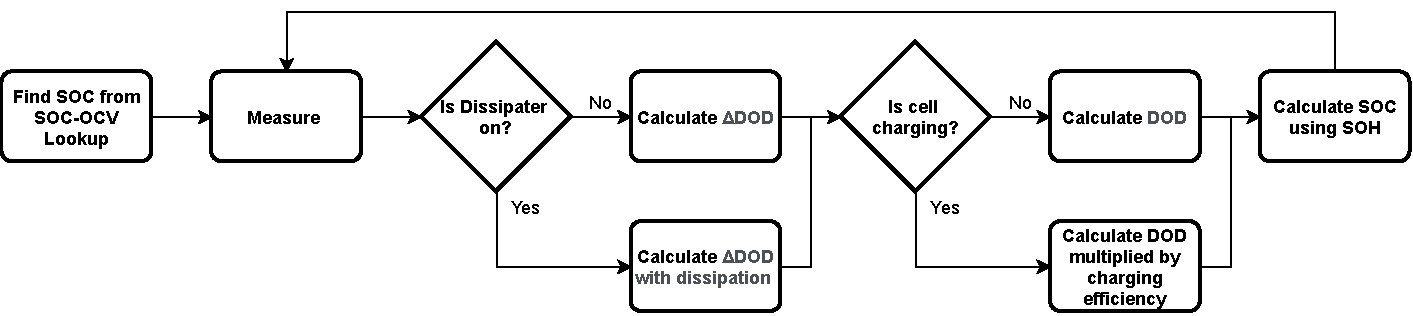
\includegraphics[scale = 0.7]{ColoumbCounting (2).pdf}
    \caption{Top level SOC finding algorithm}
    \label{fig:SOCFlow}
\end{figure}


\noindent\begin{minipage}{.32\linewidth}
\begin{equation}
    SOC = 1 - DOD
  \label{equ:SOC}
\end{equation}
\end{minipage}
\begin{minipage}{.32\linewidth}
\begin{equation}
    SOH = \frac{Q_{Discharge}^{Max}}{Q_{Rated}}
  \label{equ:SOH}
\end{equation}
\end{minipage}
\begin{minipage}{.32\linewidth}
\begin{equation}
    \eta_c = \frac{Q_{Discharge}^{Max}}{Q_{Charge}^{Max}}
  \label{equ:ChargeEfficiency}
\end{equation}
\end{minipage}

In (\ref{equ:SOC}), the state of charge can be represented as a decimal or a percentage. It is a measure of the current capacity of the cell. The state of health (\ref{equ:SOH}) is defined as the maximum discharge capacity compared to the rated capacity of the cell. It can also be represented as a percentage of the rated capacity. The charge efficiency (\ref{equ:ChargeEfficiency}) is used to create a more accurate Coulomb counting algorithm whereby the increased capacity needed during charging is accounted for as seen in figure \ref{fig:SOCFlow}.   

\noindent\begin{minipage}{.49\linewidth}
\begin{equation}
    \Delta DOD = \frac{I_{Bat}}{3600*SOH*Q_{Rated}}
  \label{equ:DeltaDOD}
\end{equation}
\end{minipage}
\begin{minipage}{.49\linewidth}
\begin{equation}
    DOD_{(k+1)} = DOD_{(k)} - \eta\Delta DOD
  \label{equ:DOD}
\end{equation}
\end{minipage}

In discrete one second intervals, $\Delta DOD$ (\ref{equ:DeltaDOD}) is seen to be the amount of amp-hours in the sampling period compared to the maximum discharge capacity which has been expanded to include the SOH. During charging, the next value of depth of discharge (\ref{equ:DOD}) decreases with an $\eta = \eta_c$. Conversely, the DOD increases during negative current (Out of cell) with $\eta=1$.

\textbf{Arduino - SOH Maintanance}

The state of health decreases as the number of charge-discharge cycles begins to accumulate. Hence it is important to track to ensure an accurate Coulomb Counting algorithm. This can be done by calibrating the SOH and $\eta_c$ during a full charge/discharge (\ref{fig:RecalibrationAlgorithm}). This was done during the characterisation of each cell. Ideally this would happen after 1-2 full charge-discharge cycles which would allow the coulomb count to zero itself. To prolong the life of a cell in a battery pack, an SOH maintenance strategy must be employed. This is needed to prevent a single, smaller cell, from restricting the larger cells from charging to maximum capacity. The smaller cell would then degrade at a faster rate than the others leading a lower overall battery capacity. This strategy involves developing a system to keep the various SOCs at around the same level. There are a range of balancing strategies open to us. The simplest and most effective is passive cell balancing. This involves using dedicated dissipation resistors through which the individual cells can discharge to lower their respective SOC to that of the whole battery pack. This seemed like the most obvious option given the already implemented dissipation resistors in the battery PCBs. The balancing algorithm was then idealized shown by the flowchart in figure \ref{fig:DisAlgorithm}. It should be noted that the cells should stop dissipating when they are within 3\% of its other due to the SOC only being an estimation

\begin{figure}[hbt]
    \centering
    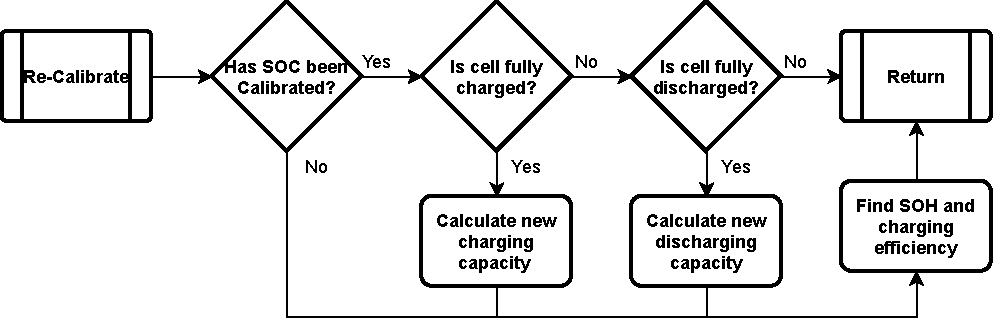
\includegraphics[scale = 0.7]{Recalibration (1).pdf}
    \caption{Re-calibration algorithm}
    \label{fig:RecalibrationAlgorithm}
\end{figure}

\noindent\begin{minipage}{.49\linewidth}
\begin{equation}
    Q^{Max}_{{Charge}_{(k+1)}} = \frac{SOC - SOC_{Init}}{DOD_{Init}}Q^{Max}_{{Charge}_{(k)}}
    \label{equ:NewChargingCap}
\end{equation}
\end{minipage}
\begin{minipage}{.49\linewidth}
\begin{equation}
    Q^{Max}_{{Discharge}_{(k+1)}} = \frac{SOC_{Init} - SOC}{SOC_{Init}}Q^{Max}_{{Discharge}_{(k)}}
    \label{equ:NewDischargingCap}
\end{equation}
\end{minipage}

Equation \ref{equ:NewChargingCap} states that the new value of the maximum charge capacity is the ratio of the actual DOD at full capacity compared to the initial estimated DOD multiplied by the old value for the maximum capacity. Hence, if the real DOD was lower than estimated, a smaller value of charge capacity is calculated. This can then be used to find a new $\eta_c$ (\ref{equ:ChargeEfficiency}). Similarly, (\ref{equ:NewDischargingCap}) calculates a new discharge capacity by using the ratio of the actual DOD and the initial SOC. This is then applied to the previous value of the discharge capacity. Through this, a re-calibration of the SOH (\ref{equ:SOH}) and $\eta_c$ (\ref{equ:ChargeEfficiency}) can be processed.
\begin{figure}[hbt!]
    \centering
    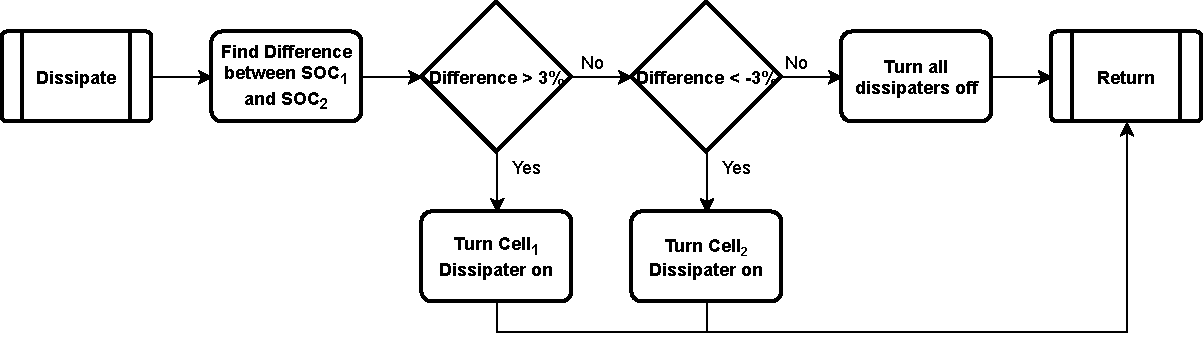
\includegraphics[scale = 0.7]{Dissipate (3).pdf}
    \caption{Dissipation algorithm}
    \label{fig:DisAlgorithm}
\end{figure}

\textbf{Arduino - PV MPPT Algorithm}

PV panels produce a non-linear voltage-current curve which can vary significantly with temperature and luminosity. This multiplied by the changing efficiency of the SMPS leads to a non-linear, dynamic power curve (\ref{CharPVPanel}) which needs to be taken advantage of in order to get the maximum power output. It was decided that Incremental Conductance  would be used as the MPPT algorithm due to low fluctuations at the peak. The strategy works by making a linear estimation of the gradient using the past sample value as seen in (\ref{fig:Gradient}) and following the flowchart seen in figure \ref{fig:IncrementalConductance}. A positive gradient would mean that the system is on the left hand side of the peak and vice versa for a negative gradient. The function would then change the duty cycle accordingly to change the impedance of the power supply as seen by the PV panel. The MPPT program also tracks if the irradience has changed which would result in no change in voltage but a change in current. 
\begin{equation}
    \frac{dP}{dV} = \frac{d(VI)}{dV} = I + \frac{dI}{dV} \approx I + \frac{\Delta I}{\Delta V}
    \label{fig:Gradient}
\end{equation}

\begin{figure}[hbt!]
    \centering
    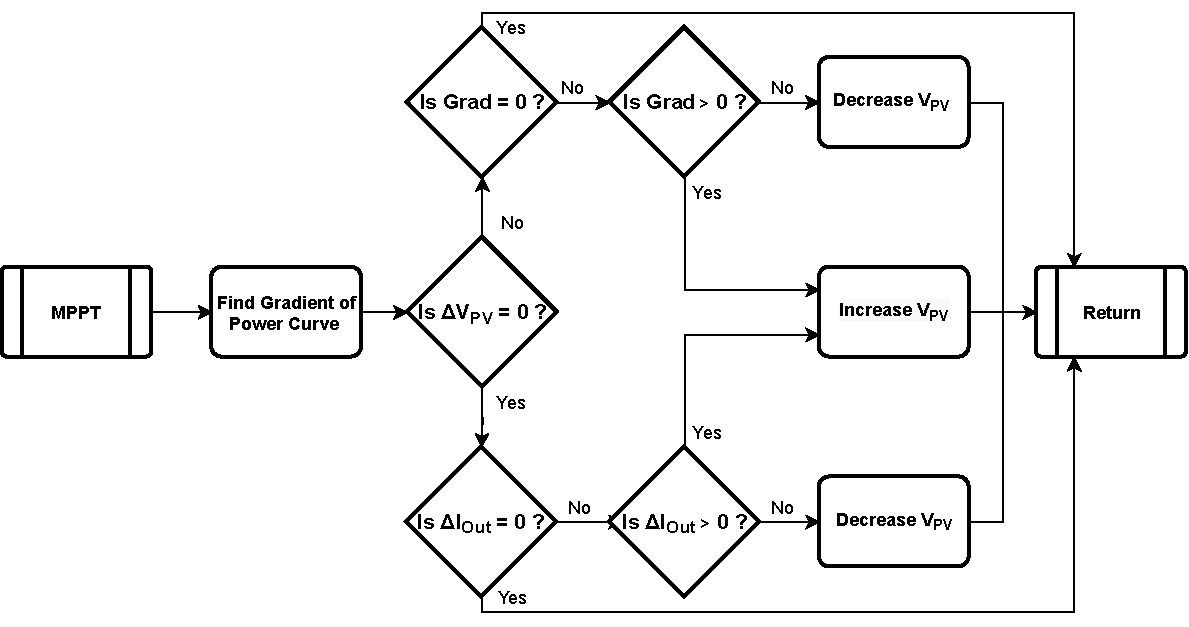
\includegraphics[scale = 0.7]{IncrementalConductance2 (2).pdf}
    \caption{Incremental Conductance Algorithm \quad Source: Adapted from \cite{Choudhary2014IncrementalConverter}}
    \label{fig:IncrementalConductance}
\end{figure}

\textbf{Arduino - Communication}

Communication between Energy and the rest of the subsystems is important in the reliability of the rover. The SOC, SOH, Rover Range and Low Battery Flag will be sent to control which will relay these to Command. The SOC will be that of the lowest cell and the SOH will be the average of both cells. To get an accurate SOC and Rover Range, the overall current drawn and speed of the rover must be received by Energy. Lastly, Command must send a Charge Flag to indicate that the rover is connected to the solar charging station. 

\textbf{Arduino - Cell Safety}

The use of LiFePO cells requires stringent safety protocols. Based upon the cell specification (Appendix \ref{appendix:Energy}.\ref{tab:EnergySpec}) and the maximum values in table \ref{tab:EnergySpec}, the energy subsystem will completely shut down and refuse to give power unless the problem is solved. This will be done with the use of relays which will disengage the cells.

\textbf{Arduino - Rover Range}

The rover range is found using (\ref{equ:RoverRange}). This will provide an estimate given the speed, SOC and current draw. The equation will be adjusted according to the SOH; keeping the estimate accurate as the cycle count of the battery pack increases.   
\begin{equation}
    Range = \left(\frac{Q_{Discharge}^{Max}}{I_{Out}}3600\right) v_{rover} = \left(\frac{SOC \ SOH \ Q_{Rated} }{I_{Out}} 3600\right) v_{rover}      
    \label{equ:RoverRange}
\end{equation}

\textbf{SMPS - Initial Top Level Design}

How the Energy subsystem is integrated within the design of the rover is more of a hypothetical problem. The processing on board requires a reliable 5V supply which would require the use of another SMPS to step down the voltage of the cells. In our case, the battery is only used to power the motor control through a connection to Port A of the Drive SMPS as seen in figure \ref{fig:InitalDesign}. The drive current is needed to work out the actual current going through the battery for the SOC and range calculations.

\begin{figure}[hbt]
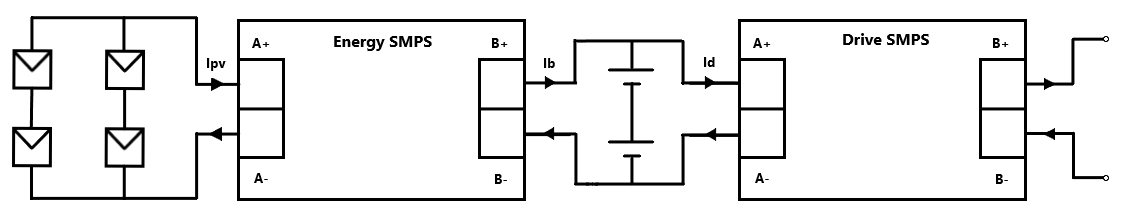
\includegraphics[scale = 0.55]{SMPS}
\centering
\caption{Preliminary design for connection to drive subsystem}
\label{fig:InitalDesign}
\end{figure}

\textbf{Battery Pack - Configuration}

It was decided that safety and good cell maintenance would be a priority when deciding on the configuration of the cells. This led to the series design seen in figure \ref{fig:InitalDesign}. The series battery pack has the advantage that one can always monitor the current going through each cell which can then be used to ensure the battery is not damaged through over charging/discharging. Unfortunately, more than two cells in series is not possible with the SMPS in synchronous mode due to a $\approx 8V$ limit on port A. This is a limitation of the PMOS MOSFET's Gate threshold voltage and more cells cannot be added as the Drive SMPS requires a buck configuration (Hence the PMOS cannot be set as a diode) 

\textbf{PV Panels - Configuration}

One can see the classic characteristic PV curves on figure \ref{fig:PVChar}. The PV specification (Appendix \ref{appendix:Energy}.\ref{tab:PVSpecification}) states that the voltage of the PV panel is 5V. As seen in figure \ref{fig:InitalDesign}, a 2x2 design ensures that the PV voltage is above that of the battery pack. Like before, the input voltage limit of the SMPS will affect this arrangement. During testing it worked but a series configuration is impossible as a buck is required from the SMPS.

\textbf{Final State Machine}

The final state diagram can be seen in figure \ref{fig:FinalState}. It should be noted that the various functions such as \textit{Dissipate} and \textit{SOC} stated above run every cycle and so have not been included in the figure.  

\begin{figure}[hbt]
    \centering
    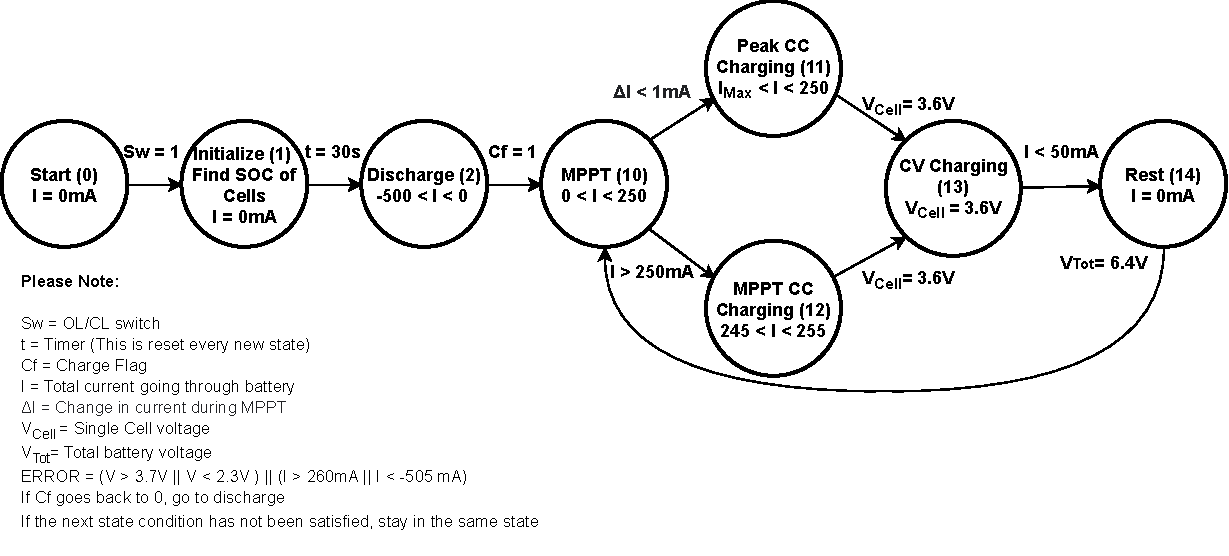
\includegraphics[width = \textwidth]{Final (2).pdf}
    \caption{Final State Machine}
    \label{fig:FinalState}
\end{figure}

\newpage
\subsection{Vision}

\textbf{Edge detection implementation:}

We use edge detection to provide more advanced data for obstacle avoidance and route planning . As well as to corroborate the hue analysis that occurs in ball detection. This provides us with a more detailed image of the environment. 

Video data is received from the camera as a continuous stream of pixels or frame packet information. The edge detection process analyses the valid pixels of this stream for each frame forming an edge detected video stream which is analysis can be derived from. Each pixel received is in an RGB format. Where R,G and B are represented by a byte having a value between 0 and 255 . 

The first step in the edge detection process is to calculate the luminance of each pixel from its RGB values. Lumianance or Luma is an important photo-metric measure describing the brightness of a pixel it is often used to produce an achromatic image giving us a more meaningful visual space to extract meaning from. I followed an approximation for the digital CCIR 601 \verb|(ADD REFERENCE https://en.wikipedia.org/wiki/Luma_(video))| video standard. This value will be between 0 and 255 and be a weighted sub of the R , G , B values of the pixel. 

\begin{minipage}{.49\textwidth}
\begin{equation}
    Y_{601} = 0.299R + 0.587G + 0.114B
\end{equation}
\end{minipage}
\begin{minipage}{.49\textwidth}
\begin{equation}
    Y_{Approx} = 0.375R + 0.5G + 0.125B
\end{equation}
\end{minipage}

We use an approximation as such specific fractions cannot be represented easily as a series of additions and bit shifts in Verilog  without the addition of a large amount of complexity. It was accepted that the small reduction in accuracy was acceptable for our application. As later a threshold would be applied with would highlight low and high lumiances for ease of analysis. 

Following review of the luminance space image , i observed a large amount of speckled noise like data.I decided the removal of this data through some Gaussian filtering would give me a smoothed luminance space removing an erratic brightness data that may be present in the luminance space. To accomplish this it was necessary to apply a Gaussian filter to the luminance space. This was accomplished though convolution of a 1D Gaussian kernel with a series of horizontal pixels. And returning a Gaussian value which is the convultion product for that specific pixel. See reference \verb|https://homepages.inf.ed.ac.uk/rbf/HIPR2/gsmooth.html| 

\begin{figure}[hbt]
    \begin{minipage}{.55\textwidth}
    \begin{equation}
        \begin{bmatrix}
        0.006 & 0.061 & 0.242 & 0.383 & 0.242  & 0.061  & 0.006 \\
    \end{bmatrix}
    \end{equation}
    \end{minipage}
    \begin{minipage}{.39\textwidth}
    \begin{equation}
        \begin{bmatrix}
        0.0625  & 0.25 & 0.375 & 0.25  & 0.0625 \\
        \end{bmatrix}
    \end{equation}
    \end{minipage}
    \caption{1D x component Gaussian Kernel (12)  and  approximated version (13)}
\end{figure}

To accomplish convolution i store the current and previous four values of pixel luminances in a buffer called Guassian\verb|_|buffer , after storing these values i calculate the sum of weighted values in the buffer weighting is accomplished through bit shifting each luminance value according to its position. The weighting values are again approximated as shown above to an acceptable degree of accuracy. Thus the kernel moves through the image data horizontally. The sum of weighted luminances is then returned as a gaussian value in a new stream.

\begin{figure}[hbt]
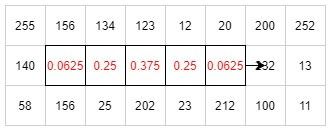
\includegraphics[scale = 0.55]{GaussianBufferjpg.jpg}
\centering
\caption{Gaussian buffer example}
\label{fig:InitalDesign}
\end{figure}

After this convolution i now have a Gaussian filtered luminance video stream which is ready for edge detection

\newpage

I attempted two methods when implementing edge detection on the Gaussian filtered luminance video stream. The first being a 3x3 kernel applied across and the second a 1X5 horizontal Sobel filter. Both methods had their benefits and drawbacks which will be discussed. 

\textit{Method 1 - 3X3 Kernel}

To apply the following kernel it is necessary to have on access the values under the matrix , this stretches across three rows of pixels and three columns.These values are not accessible from the stream so we must create a buffer which stores the previous pixels of the stream making them accessible for the matrix convolution. I attempted to implement this buffer with a bank of registers defined as such:

reg [7:0] luminance\verb|_|buffer[2:0][(IMAGE\verb|_|W-1):0] 

This stores the RGB values for all pixels in the three rows necessary. However this implementation took exceedingly long to compile. I then attempted a version using a shift register IP block in the QSYS however i stopped developing this method before the shift register was fully implemented as i decided upon using method two.

Thus the matrix convolution will can be calculated as such :
\begin{minted}{verilog}

assign GXSOBEL = (1 * ImageMatrix[2][0] ) + (-1 * ImageMatrix[2][2] ) + 
(2 * ImageMatrix[1][0] ) + (-2 * ImageMatrix[1][2] ) + 
(1 * ImageMatrix[0][0] ) + (-1 * ImageMatrix[0][2] )

assign GYSOBEL = (-1 * ImageMatrix[2][0] ) + (-2 * ImageMatrix[2][1] ) + 
(-1 * ImageMatrix[2][2] ) + (1 * ImageMatrix[0][0] ) + (2 * ImageMatrix[0][1] ) + 
(1 * ImageMatrix[0][2] )

\end{minted}
The value GSOBEL was then calculated from GXSOBEL and GYSOBEL in the following way: 
\begin{minted}{verilog}
assign GSOBELSQUARED = ((GYSOBEL)*(GXSOBEL)) + ((GYSOBEL) * (GYSOBEL)) 
assign GSOBEL = sqrt(GSOBELSQUARED)
\end{minted}

\begin{figure}[!htb]
\begin{minipage}{.49\textwidth}
        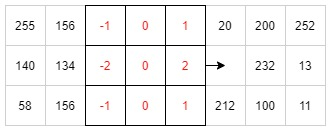
\includegraphics[scale = 0.55]{GX.jpg}
        \centering
        \caption{Horizon}
        \label{fig:InitalDesign}
\end{minipage}
\begin{minipage}{.49\textwidth}
        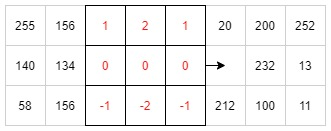
\includegraphics[scale = 0.55]{GY.jpg}
        \centering
        \caption{Gaussian buffer example}
        \label{fig:InitalDesign}
\end{minipage}
\end{figure}



\begin{figure}[hbt]
    \begin{minipage}{.33\textwidth}
    \begin{equation}
    G_{X} =
        \begin{bmatrix}
        -1 & 0 & 1 \\ 
        -2 & 0 & 2 \\
        -1 & 0 & 1 \\
    \end{bmatrix}
    \end{equation}
    \end{minipage}
    \begin{minipage}{.33\textwidth}
    \begin{equation}
         G_{Y} =
        \begin{bmatrix}
        1 & 2 & 1 \\ 
        0 & 0 & 0 \\
        -1 & -2 & -1 \\
    \end{bmatrix}
    \end{equation}
    \end{minipage}
     \begin{minipage}{.33\textwidth}
    \begin{equation}
    G = \sqrt{G_{X}^2 + G_{Y}^2}
    \end{equation}
    \end{minipage}
    \caption{3X3 Sobel Kernel for horizontal and vertical and final}
\end{figure}

I chose not to use this method because of a few issues .Firstly the implementation revels both horizontal and vertical edges in the image, however i discovered that only vertical edges are of concern to our rover for avoiding obstacles this is because vertical edges highlight the left and right edges of obstacles which must be avoided. As such it was unnecessary to calculate GX and GSOBEL as they would not be used analysis. Therefore to reduce the complication of design and any usage of unnecessary FPGA hardware i followed method 2. Further to this memory buffer / shift register used was very large in the current design which led to considerable delay in compilation and increased risk of propagation delay IS THIS TRUE?. 

\newpage


\textit{Method 2- 1X5 horizontal Kernel}

The second method is relatively simpler than the first as we use  a 1D horizontal kernel which  means we must only store the current and four previous pixel RGB values for our convolution calculation. However this method requires us to orient the camera horizontally but results in far simpler buffer and convolution implemented as such (where Gaussian is the filtered stream pixel):

\begin{figure}[hbt]
\begin{minipage}{.56\textwidth}
\begin{minted}{verilog}
reg [10:0] luminance_buffer[4:0];
always@(posedge clk) begin
    luminance_buffer[4] <= {3'd000,Gaussian}; 
	luminance_buffer[3] <= luminance_buffer[4]; 
	luminance_buffer[2] <= luminance_buffer[3]; 
	luminance_buffer[1] <= luminance_buffer[2]; 
	luminance_buffer[0] <= luminance_buffer[1];
end
assign GSOBEL = luminance_buffer[0] + luminance_buffer[1] 
           + ~luminance_buffer[3] + ~luminance_buffer[4]; 
\end{minted}
\end{minipage}
\begin{minipage}{.42\textwidth}
            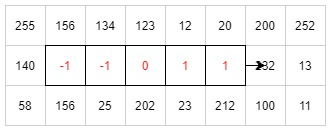
\includegraphics[scale = 0.4]{Method2Matrix.jpg}
            \centering
            \caption{1D Sobel kernel visualisation}
            \label{fig:InitalDesign}
\end{minipage}
\end{figure}

\textit{Horizontal camera orientation and highlighting}

ASK MAX

\textit{Analysis of highlighted edge video stream}

We then analyse the edge video stream in the following way : First the height of the image was divided into  80 vertical sections, each section has a sum and count which is reset when we enter a new section. When a white pixel is defected in this vertical section we add the vertical position of the white pixel to the sum and increment the count. At the end of the section we divide the sum by the count then inputting this result into the memory array for communication to the Command subsystem. When the final section is complete we reset the sum and count for the next frame. This process is done for only part of the image excluding data at the top of the camera as it is visually too far from the rover. 

\textbf{Communication to control subsystem:}

To communicate with the arduino we are connected via 3 GPIO pins which we use to implement a basic SPI communication protocol  . The pins are select , MISO and clkArduino . when select is low the arduino begins to request data from the FPGA when select is high is is not requesting. The miso line is the avenue which the bit stream of data from the memory array will flow. The memory array is a bank 98 registers storing 1 byte each. The first memory register is loaded with an open message symbol \verb|'{'| in ascii 123 and the 98th register is a close message symbol \verb|'}'| in ascii 125. The memory bank is read from 1 register at a time from start to finish where on each block pulse the next bit is read. With byte and bit addresses being updated for as we move through the registers. The implementation can be seen below and is relatively simple: 

\textit{Register map :} 0 = open message symbol , 1-15 = ball ids and bounding mins and max , 16-96 = avg height of edge in section starting from left to right, 97 = close message symbol . 

\begin{minted}{verilog}
always @(posedge clkArduino) begin
if ( selectArduino == 0)begin
  miso  <= (counterByteAddress < 7'd100) ? mem[counterByteAddress][counterBitAddress] : 0 ;
  counterBitAddress <= counterBitAddress + 3'b1 ;
  counterByteAddress <= counterByteAddress + (counterBitAddress == 3'b111);
end    
if ( selectArduino == 1)begin
  miso <= 0 ;
  counterBitAddress <= 3'b0 ;
  counterByteAddress <= 7'b0;
end
end

\end{minted}

\newpage

\textbf{Ball detection Implementation:}

Each ball is detected using the same process using modified thresholds. The process begins by converting the RGB space into a highlighted HUE space representation. According to the HUE regions we assign either a white or black value to the pixel. For example, if the RGB values of the pixel lie in the orange HUE region we set the HUE\verb|_|Orange value to 0 for black. If it does not lie in this region we set it to 255 for white. This process is implemented as such:

\begin{figure}[hbt]
\begin{minipage}{.54\textwidth}
\begin{minted}[fontsize=\footnotesize]{verilog}
reg  [7:0]HUE_Orange ; 
always@(posedge clk) begin
if(R >= G)begin 
	if(R >=  B)begin  // R > G  && R > B, R IS MAX
		if (G >= B )begin // R MAX B MIN
			HUE_Orange <=  8'd0; 
		end 
		else begin // R MAX G MIN
			HUE_Orange <=  8'd255; 
		end
	end
end
//Implementation is cut here as too long but can be 
            //found in appendix
\end{minted}
\end{minipage}
\begin{minipage}{.45\textwidth}
            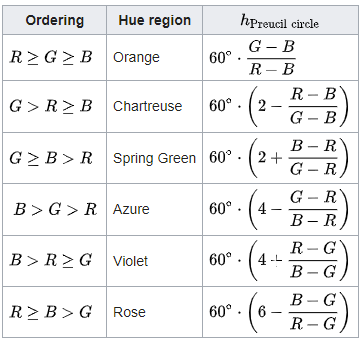
\includegraphics[scale = 0.4]{HueRegions.PNG}
            \centering
            \caption{HUE region table}
            \label{fig:InitalDesign}
\end{minipage}
\end{figure}

However some noise/unexpected RGB value exist which disrupts the bounding which occurs later. This to filter stray highlighted pixels that speckle across the image, we have a very simple filtering process. We use a buffer to store the current and previous 4 highlighted HUE values of the pixels (Using a buffer process shown below) . We then examine the top bit of this values, If its 0 then it will be highlighted and if its 1 its not, Thus if all stored pixel HUE values are 0 then all are highlighted and we accept this is not noise but a consistent region of orange/black/pink hue. As such we then re-highlight this pixel as white (Implying non noise) and black if it is noise. This leaves us with a image as such:

\begin{figure}[hbt]
\begin{minipage}{.49\textwidth}
\begin{minted}[fontsize=\footnotesize]{verilog}
wire  Orange_detect  ; 
assign Orange_detect = ~HUE_Orange_buffer[4][7] 
                    && ~HUE_Orange_buffer[3][7] 
                    && ~HUE_Orange_buffer[2][7] 
                    && ~HUE_Orange_buffer[1][7] 
                    && ~HUE_Orange_buffer[0][7]  ; 
wire [23:0] HUE_Out_Orange  ;
assign HUE_Out_Orange = {Orange_detect, ... ,Orange_detect} ; 

\end{minted}
\end{minipage}
\begin{minipage}{.49\textwidth}
            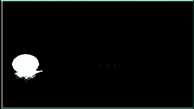
\includegraphics[scale = .99]{Detect.PNG}
            \centering
            \caption{Highlighted detected image (Orange)}
            \label{fig:InitalDesign}
\end{minipage}
\end{figure}

We now apply the simple bounding box process upon this filtered highlighted hue space The values of Ymin , Ymax and Xmin Xmax for each ball are updated at the eop for each frame. This method works relatively robustly but can be affected by high contrast conditions. As such we keep our camera in a low contrast / low brightness mode when bounding the boxes which seems is a preferable environment. 

\begin{figure}[hbt]
    \centering
    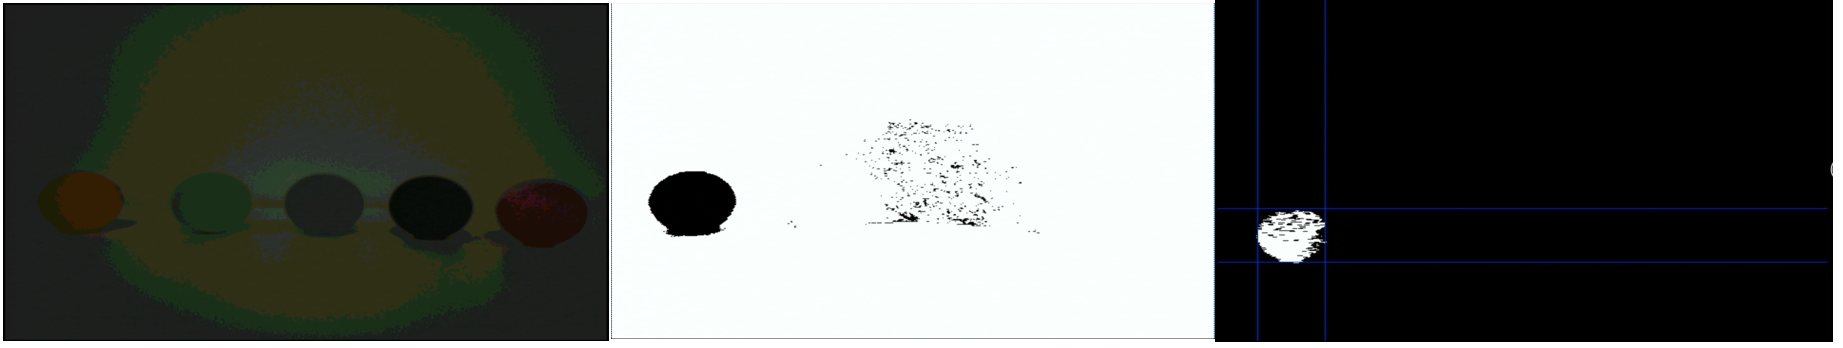
\includegraphics[scale = 0.35]{AnalysisImag.PNG}
    \caption{Highlighted Hue space before and after noise filtering}
    \label{fig:HightedHueSpace}
\end{figure}



\newpage

\subsection{Command}

\subsection{Control}
\textbf{Data Timing}
The ESP32 is what controls and manages the flow of information. It collects data from every subsystem, sends it to the server for processing and finally receives back data to reach the next destination.
\smallbreak
In particular the flow of information proceeds as follows:
\begin{figure}[hbt!]
    \centering
    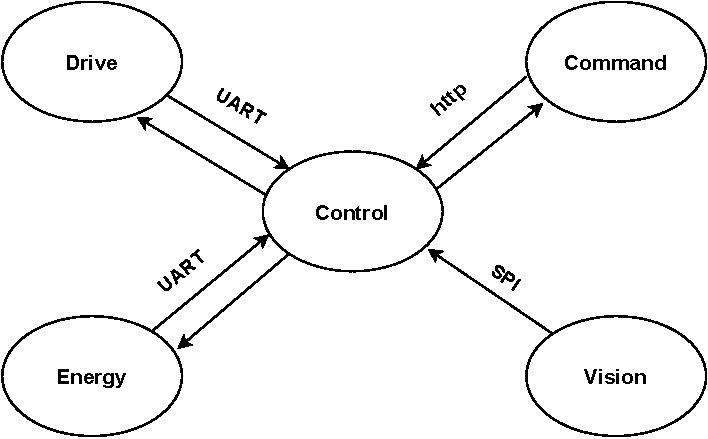
\includegraphics[scale=0.35]{esp32_comms.pdf}
    \captionsetup{justification=centering}
    \caption{High Level data flow}
\end{figure}

\medskip

\textbf{receive and send data}
In order to communicate with the Drive, Vision and Energy subsystems a general message protocol has been designed to ensure that only valid data is received. The message is composed by:
\begin{itemize}
    \item a Start of Message character, used to identify the beginning of the message
    \item the payload of the message. The size and structure of the payload is fixed and depends on the specific subsystem considered.
    \item an End of Message character, used to identify the end of the message
\end{itemize}

The Arduino code used to receive messages in this form is:
\begin{minted}[fontsize=\footnotesize]{C++}
void receive_data_Drive()
{
    static bool recvInProgress_Drive = false;
    static byte counter_Drive = 0;
    char SOM = '{';
    char EOM = '}';
    char received_byte;

    while (true)
    {
        while (Serial2.available() > 0)
        {
            received_byte = Serial2.read();
            //discard bytes until SOM is encounterd
            if (received_byte == SOM)
            {
                recvInProgress_Drive = true;
                continue;
            }

            //receive data
            if (recvInProgress_Drive == true)
            {
                if (received_byte == EOM)
                {
                    recvInProgress_Drive = false;
                    counter_Drive = 0;
                    return;
                }
                receivedData_Drive[counter_Drive] = received_byte;
                counter_Drive++;
            }
        }
    }
}

\end{minted}








Different communication protocols have been chosen to meet the design criteria

\paragraph{UART} The UART communication protocol has been chosen for data transmission between Drive and Control and between Energy and Control. 
The biggest challenge in the Control subsystem was to allow fast bi-directional communication between Energy and Control. The bottleneck was the presence of interrupts in the Energy code, dindn't allow delays introduced by receiving data (stalling the system) for communication.
Our solution to the problem was to: pick-full duplex communication protocol, use second core of esp32 

In particular UART was chosen because: 
\begin{itemize}
    \item it allows full-duplex (I2C doesn't)
\end{itemize}


\paragraph{SPI} The SPI communication protocol has been chosen for data transmission between Vision and Control.
%%%%% maybe add about verilog code + spi library %%%%%%
In particular SPI was chosen because: 
\begin{itemize}
    \item it allows for high speed data transmission and is faster than UART or I2C. This makes it suitable for transmitting large amount of data such as image data received from Vision 
    \item it provides robust error detection features
\end{itemize}


\paragraph{http} http GET and POST requests have been chosen for data transmission between Command and Control.



\newpage


\section{Testing and Evaluation}
\subsection{Testing and analysis}

\subsubsection{Drive}

Functionality of each drive implementation was tested by hard coding target distances and target angles in all four quadrants and observing the behaviour of the rover.

Precision and accuracy of each implementation was tested and compared in order to choose the final implementation. Testing was carried out using the whole rover to account for any effects that loading from the control and vision subsystems might introduce.









\subsubsection{Energy}

Dont worry there will be two side-by side

\begin{figure}[hbt!]
  \centering
  \begin{minipage}[b]{0.49\textwidth}
    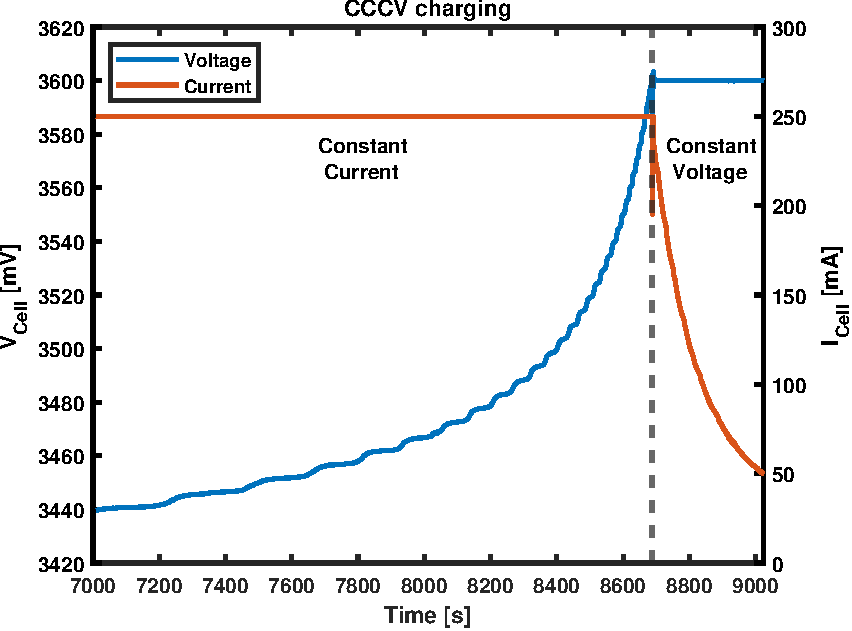
\includegraphics[width=\textwidth]{CCCV.pdf}
    \caption{Constant Current - Constant Voltage charging}
    \label{fig:TestCCCV}
  \end{minipage}
  \hfill
  \begin{minipage}[b]{0.49\textwidth}
    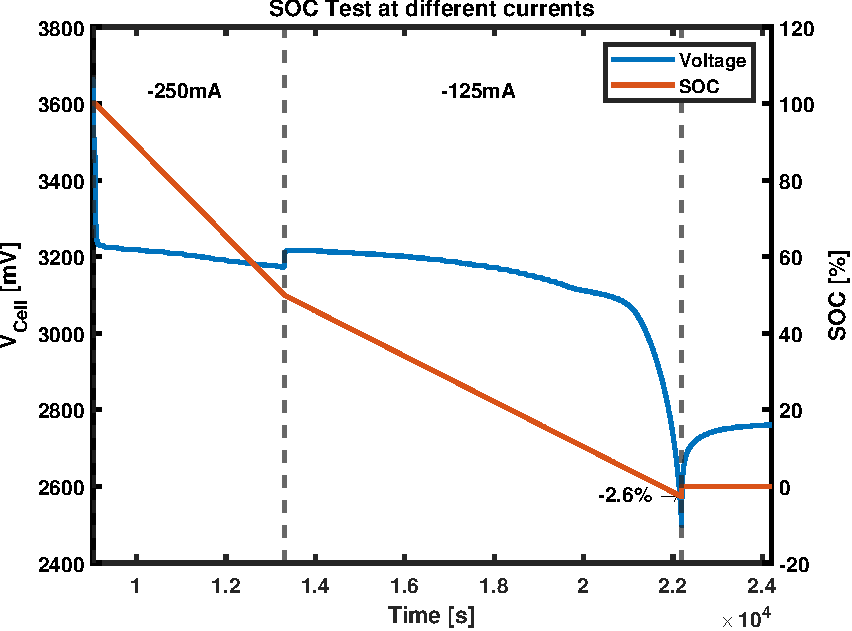
\includegraphics[width=\textwidth]{SOC.pdf}
    \caption{SOC discharge at different currents}
    \label{fig:TestSOC}
  \end{minipage}
\end{figure}

\begin{figure}[hbt!]
  \begin{minipage}[b]{0.46\textwidth}
    \centering
    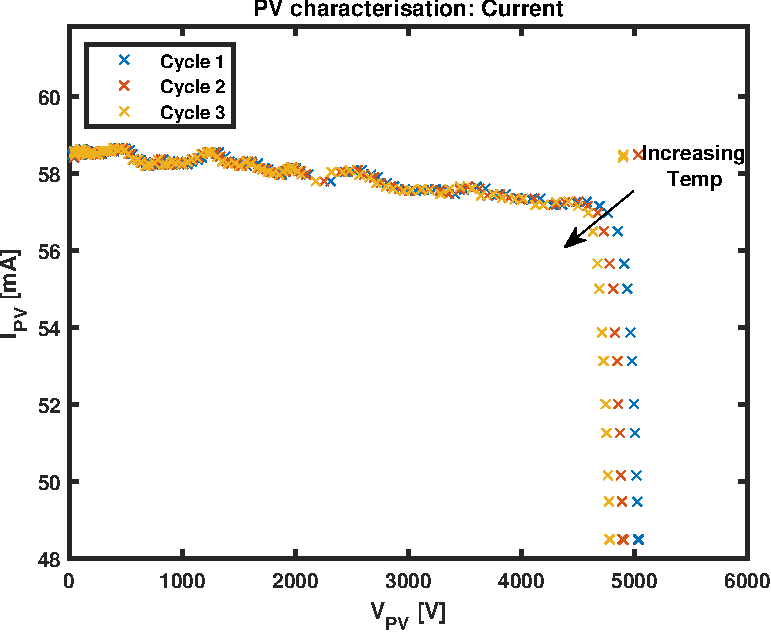
\includegraphics[width=\textwidth]{PVvoltage.pdf}
    \caption{PV Current Characterisation}
    \label{fig:PVvoltage}
  \end{minipage}
  \hspace{0.7cm}
  \begin{minipage}[b]{0.46\textwidth}
    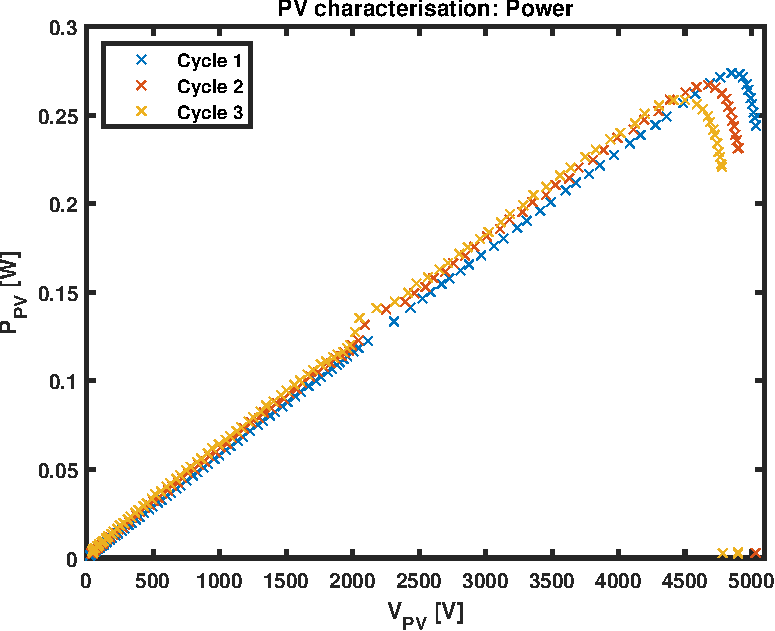
\includegraphics[width=\textwidth]{PVpower.pdf}
    \caption{PV Power Characterisation}
    \label{fig:PVpower}
  \end{minipage}
\end{figure}

\subsubsection{Vision}

\subsubsection{Command}

\subsubsection{Control}

\subsubsection{Integration}

\subsection{Critical Analysis / Evaluation}

\subsubsection{Drive}

\subsubsection{Energy}

\subsubsection{Vision}

\subsubsection{Command}

\subsubsection{Control}

\subsubsection{Integration}

\section{Reflection}

\section{Essay 'Intellectual Property'}




\newpage
\begin{appendices}

\section{Energy}

\setcounter{figure}{0}  %Resets the figure count
\setcounter{table}{0}   %Resets the table count



\begin{table}[htb]
    \centering
    \renewcommand{\arraystretch}{1.3}
    \begin{tabular}{||c|c|c||}
    \hline
    Specification & Value & Unit \\ [0.5ex]
    \hline \hline
    Nominal Voltage    & 3.2 & V\\
    Nominal Capacity     & 500 & mAh\\
    Minimum Voltage         & 2  & V\\
    Charging Method     & CC/CV 3.6  & V\\
    Standard Charging Current CC    & 250  & mA\\
    Continuous Discharge Current   & 500  &   mA\\
    \hline
    \end{tabular}
    \caption{Cell Specification \quad Source: Adapted from \cite{AmpsplusBattery}}
    \label{fig:CellSpecification}
\end{table}
\label{appendix:Energy}

\begin{table}[htb]
    \centering
    \renewcommand{\arraystretch}{1.3}
    \begin{tabular}{||c|c|c||}
    \hline
    Specification & Value & Unit \\ [0.5ex]
    \hline \hline
        Voltage  & 5 & V\\
        Current & 230 & mA\\
        Power & 1.15 & W \\
        Power Tolerance & +/-3 & \% \\
        Temperature Coefficient & -0.45 & $\circ C$ \\
        \hline
    \end{tabular}
    \caption{PV Specifiation \quad Source: Adapted from \cite{NoTitle}}
    \label{tab:PVSpecification}
\end{table}

\end{appendices}

\bibliographystyle{IEEEtranN}
\bibliography{references.bib}












\end{document}
